\documentclass[11pt,letterpaper]{article}
\usepackage[utf8]{inputenc}

%----- Configuración del estilo del documento------%
\usepackage{epsfig,graphicx}
\usepackage[left=2cm,right=2cm,top=1.8cm,bottom=2.3cm]{geometry}
\usepackage{fancyhdr}
\usepackage{lastpage}
\usepackage{url}
\pagestyle{fancy}
\fancyhf{}
\rfoot{\textit{Página \thepage \hspace{1pt} de \pageref{LastPage}}}


%------ Paquetes matemáticos básicos --------%
\usepackage{amsmath}
\usepackage{amssymb}
\usepackage{amsthm}

\usepackage[spanish]{babel}
\usepackage{graphicx}
\usepackage{hyperref}

\usepackage{tabularx}
\usepackage{xcolor}
\usepackage[table]{xcolor}
\usepackage{colortbl}
\usepackage{array, multirow, multicol, tabularx}
\usepackage{tcolorbox}
\newtheorem{theorem}{Theorem}[section]
\newtheorem{corollary}{Corollary}[theorem]
\newtheorem{lemma}[theorem]{Lemma}

%------si-------%
\definecolor{B}{HTML}{FFFFFF}
\definecolor{G}{HTML}{5e5e5e}
\definecolor{R2}{HTML}{d53d40}
\definecolor{A2}{HTML}{034190}
\definecolor{V2}{HTML}{7faa50}
\newcommand{\R}{\mathbb{R}}
\newcommand{\C}{\mathcal{C}}
\newcommand{\N}{\mathbb{N}}
\newcommand{\Z}{\mathbb{Z}}
\newcommand{\Q}{\mathbb{Q}}
\renewcommand{\theenumi}{\Roman{enumi}}
\renewcommand{\labelenumi}{{\theenumi}.}

\begin{document}

%------ Encabezado -------- %

\begin{center}
    \begin{minipage}{3cm}
    	\begin{center}
    		\includegraphics[height=3.4cm]{logo_unam.png}
    	\end{center}
    \end{minipage}\hfill
    \begin{minipage}{10cm}
    	\begin{center}
    	\textbf{\large Universidad Nacional Autónoma de México}\\[0.1cm]
        \textbf{Facultad de Ciencias}\\[0.1cm]
        \textbf{C\'alculo II}\\[0.1cm]
        Resumen del Curso\\[0.1cm]
         El\'ias L\'opez Rivera\\[0.1cm]
        \texttt{ elias.lopezr\,@ciencias.unam.mx }\\[0.1cm]
        Fecha:\,\,06/07/2025
    	\end{center}
    \end{minipage}\hfill
    \begin{minipage}{3cm}
    	\begin{center}
    		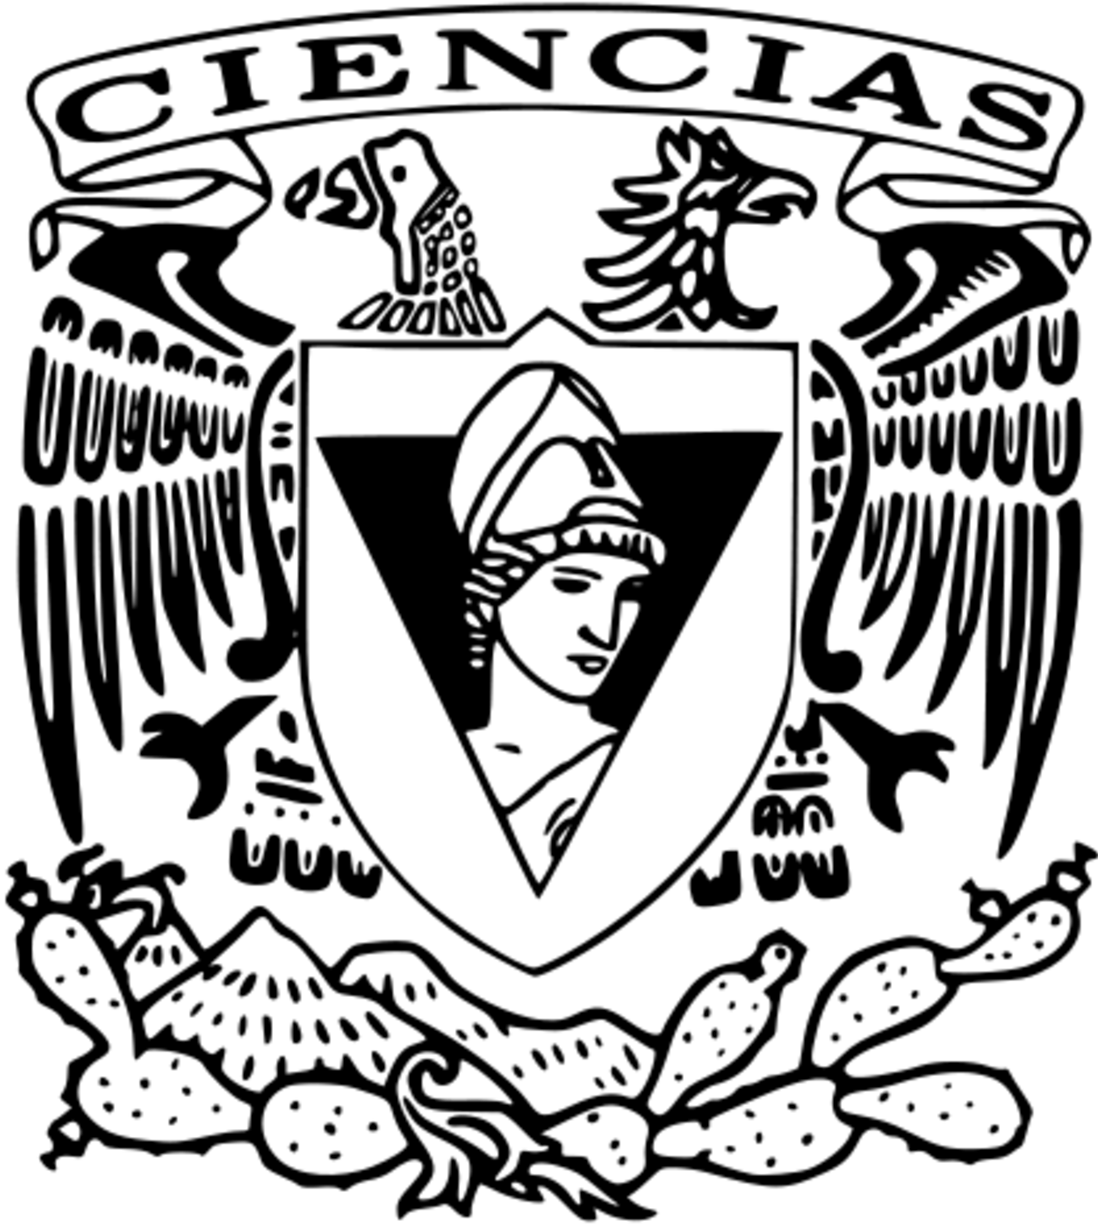
\includegraphics[height=3.4cm]{Logo_FC.png}
    	\end{center}
    \end{minipage}
\end{center}

\rule{17cm}{0.1mm}

%------ Fin de encabezado -------- %
\,\\
\begin{tcolorbox}[
	title = \textcolor{black}{\textcolor{white}{C\'alculo 2}},]
\textit{El siguiente documento es una recopilaci\'on de los teoremas,problemas de examenes,ejemplos y solcuiones m\'as 
importantes expuestos durante el curso de C\'alculo II, del profesor Javier Páez Cardeas, de la facultad de ciencias de la unam }
\end{tcolorbox}
\section*{Teorema de integrabilidad de Lebesgue}
Antes de poder demostrar este teorema necesitamos introducir 3 conceptos importantes que se usaran durante la prueba.
\subsection*{Conjuntos Nulos}
\begin{tcolorbox}[
	title = \textcolor{black}{\textcolor{white}{Definici\'on}},]
\textit{Decimos que un conjunto $A\subset \R$ es nulo si dado $\epsilon>0$, existe una coleccio\'n contable $\{(a_k,b_k)\}_{k=1}^{\infty}$, de intervalos abiertos tales que:\,\\
\,\\
\begin{equation*}
    Z\subseteq\,\bigcup_{k=1}^{\infty}\,(a_k,b_k)\,\,\,\,y\,\,\,\,\sum_{k=1}^{\infty}\,(b_k-a_k)\leq \epsilon
\end{equation*}}
\end{tcolorbox}\,\\
Partiendo de lo anterior es fácil demostrar los siguientes hechos:
\begin{tcolorbox}[
	title = \textcolor{black}{\textcolor{white}{Teorema 1}},]
\textit{\textbf{Union de conjuntos nulos}
\begin{enumerate}
    \item Si $Z_1$, $Z_2$ son conjuntos nulos entonces $Z_1\cup Z_2$ es un  conjunto nulo
\item Si $Z_n$ es un conjunto nulo para toda $n\in \N$, demostrar que $\bigcup_{n=1}^{\infty}\,Z_n$, es un conjunto nulo
\end{enumerate} }
\end{tcolorbox}
\begin{proof}\,\\
    \,\\
    \textbf{1}\,\,Tenemos que como $Z_1$ y $Z_2$ son nulos, entonces para $\frac{\epsilon}{2}>0$, existen $\{J^{1}_{k}|\,k\in \N\}$ y $\{J^{2}_{k}|\,k\in \N\}$, tales que
    $\sum_{k\in \N}\,|J^1_{k}|<\frac{\epsilon}{2}$ y $\sum_{k\in \N}\,|J^2_{k}|<\frac{\epsilon}{2}$, tenemos que $\{J^{1,2}_{k}|k\in \N\}:=\{J^1_{k}|k\in \N\}\cup\{J^2_{k}|k\in \N\}$, es un conjunto contable
    de intevalos, luego tenemos que $Z_1\cup Z_2\subset \bigcup\,_{k\in \N}\,J^{1,2}_{k}$, ademas que \\$\sum_{k\in \N}\,|J_k^{1,2}|\leq\sum_{k\in \N}\,|J^1_{k}|+\sum_{k\in \N}\,|J^2_{k}|
    \leq \frac{\epsilon}{2}+\frac{\epsilon}{2}=\epsilon$
    \newpage
    \,\\
    \textbf{2}\,\,Dada $\epsilon>0$ y $n\in \N$ existe $\{J^n_{k}|\,k\in \N\}$ tal que $Z_n\subset\bigcup_{k\in \N}\,\,J^{n}_{k}$ y $\sum_{k\in \N}\,|J^n_{k}|<\frac{\epsilon}{2^n}$, definimos\\
    $\{J^{n}_{k}|n,k\in \N\}=\bigcup_{n\in \N}\,\{J^n_{k}|k\in \N\}$, es claro que $\{J^{n}_{k}|n,k\in \N\}$ es un conjunto contable de intervalos abiertos, ademas tenemos que
    $\bigcup_{n=1}^{\infty}\,Z_n\subset\,\bigcup_{k,n\in \N}\,J^{n}_{k}$, luego finalmente tenemos que:\,\\
    $\sum_{k,n\in \N}\,|J^n_{k}|\leq \sum_{k\in \N}\,\frac{\epsilon}{2^n}=\epsilon$
\end{proof}\,\\
\begin{tcolorbox}[
	title = \textcolor{black}{\textcolor{white}{Teorema 2}},]
\textit{\textbf{Ejemplos de subconjuntos nulos}
\begin{enumerate}
    \item Si $Z\subset \R$ es finito, entonces $Z$ es nulo
\item $\Q\subset \R$ es nulo
\end{enumerate} }
\end{tcolorbox}
\begin{proof}\,\\
    \,\\
    \textbf{1}\,Se sigue del hecho de que $Z$ no tiene puntos de acumulaci\'on ,por tanto para todo $z\in \Z$ existe una vecindad $V_{x}(\epsilon)$ tal que $V_{x}(\epsilon)\cap Z-\{x\}=\emptyset$, tome estas vecindades como intervalos y rellene su coleccion contable con $\emptyset$, se dejan los detalles
    de la demostraci\'on al lector\,\\
    \,\\
    \textbf{2}\,La demostraci\'on puede encontrarse en el Bartle.
\end{proof}
\subsection*{Oscilaciones de una funci\'on}
\begin{tcolorbox}[
	title = \textcolor{black}{\textcolor{white}{Definici\'on}},]
\textit{Sea $f:A\rightarrow \R$ una funcion acotada. si $S\subset A\subset \R$, definimos la Oscilaci\'on de 
$f$ en $S$ como:\,\\
\,\\
\begin{equation*}
        W(f,S):=sup\{|f(x)-f(y)|:x,y\in S\}
\end{equation*}\,\\
Si $c\in A$, la oscilaci\'on de $f$ en $c$, se define como:\,\\
\,\\
\begin{equation*}
    w(f,c):=inf\{W(f;V_r(c)):r>0\}=\lim_{r\rightarrow 0+}\,W(f;V_r(c))
\end{equation*}}
\end{tcolorbox}\,\\
\,\\
De la definici\'on podemos deducir el siguiente teorema:
\begin{tcolorbox}[
	title = \textcolor{black}{\textcolor{white}{Teorema 3}},]
\textit{Si $f:A\rightarrow\R$ esta acotada y $c\in A$, entonces $f$ es continua en $c$ si y s\'olo si $w(f;c)=0$}
\end{tcolorbox}
\begin{proof}\,\\
    \,\\
    La demostraci\'on puede encontrarse la p\'agina 435 del Bartle, o en el repositorio de github(carpeta ESFM, bucio, lista 3, problema 27)
\end{proof}
\newpage
\begin{tcolorbox}[
	title = \textcolor{black}{\textcolor{white}{Teorema 4}},]
\textit{Si $f:[a,b]\rightarrow\R$ esta acotada, entonces $D:=\{c\in [a,b]:w(f,c)>0\}=\bigcup_{k\in \N}\,H_k$, donde 
$H_k=\{c\in [a,b]:w(f,c)>\frac{1}{2^k}\}$}
\end{tcolorbox}
\begin{proof}\,\\
    \,\\
    La demostraci\'on puede encontrarse la p\'agina 435 del Bartle, o en el repositorio de github(carpeta ESFM, bucio, lista 3, problema 27)
\end{proof}

\end{document}